\documentclass{beamer}
\newcommand{\putfig}[1]{%
	\vspace{0.8em}%
	\centerline{\includegraphics[scale=1]{./figures/#1}}%
	\vspace{0.5em}%
}
\newcommand{\separationline}{%
	\vspace{0.3em}%
	\centerline{----- $*$ ----- $*$ ----- $*$ -----}%
	\vspace{0.3em}%
}
\newcommand{\ratio}{\!:\!}
%<--------------------------------------------------------------------------->%
%%% Column %%%
\usepackage{multicol}  % \begin{multicols*}{3}[例外]字\end{multicols*}
\usepackage[english]{babel}
%<--------------------------------------------------------------------------->%
%%% Enumerate %%%
\usepackage{enumitem}
\setlist{listparindent=\parindent,parsep=0pt,nosep} % paragraph indent 
%<--------------------------------------------------------------------------->%
%%% Math %%%
\usepackage{gensymb,amssymb}
\usepackage{mathrsfs,amsmath} % \mathscr{F}
\usepackage{mathtools} % \stackrel{i.i.d.}{\sim} % \substack{-\\-} % \middle
% \usepackage{centernot}
% \usepackage{accents}
% \usepackage[makeroom]{cancel}
% \newcommand{\two}[2]{\substack{ \text{#1} \\ \text{#2} }}
% \newcommand{\raum}{\phantom{=}{\:\,}}
%<--------------------------------------------------------------------------->%
%%% Page # of # %%%
\usepackage{fancyhdr,lastpage}
\pagestyle{fancy}\renewcommand{\headrulewidth}{0pt}\fancyhf{}
\fancyfoot[C]{\footnotesize 第 \thepage\ 頁 / 共 \pageref{LastPage} 頁}
\fancypagestyle{plain}{\renewcommand{\headrulewidth}{0pt}\fancyhf{}
\fancyfoot[C]{\footnotesize 第 \thepage\ 頁 / 共 \pageref{LastPage} 頁}}
%<--------------------------------------------------------------------------->%
%%% Hyper Reference %%%
\PassOptionsToPackage{hyphens}{url}
\usepackage[hidelinks,colorlinks=true]{hyperref}
% \newcommand{\supref}[1]{\ref{#1} (p.\pageref{#1})}
%<--------------------------------------------------------------------------->%
%%% CJK %%%
\usepackage{xeCJK}
\newcommand{\chmainfont}{GenWanMin TJ L}
\newcommand{\chsansfont}{Noto Sans CJK KR Medium}
\newcommand{\chmonofont}{Noto Sans CJK KR Regular}
\setCJKmainfont{\chmainfont}[BoldFont=\chsansfont,AutoFakeSlant=0.2]
\setCJKsansfont{\chsansfont}[BoldFont=\chsansfont,AutoFakeSlant=0.2]
\setCJKmonofont{\chmonofont}
\xeCJKsetup{PunctStyle=kaiming,CheckFullRight=true}
\setlength{\parindent}{2em}
%<--------------------------------------------------------------------------->%
%%% Punctuation width %%%
\xeCJKsetwidth{、}{0.55em}
\xeCJKsetwidth{,}{0.6em}
\xeCJKsetwidth{:}{0.65em}
\xeCJKsetwidth{;}{0.65em}
\xeCJKsetwidth{。}{0.7em}
\xeCJKsetwidth{・}{0.7em}
\xeCJKsetwidth{〈〉}{0.7em}
\xeCJKsetwidth{《》}{0.7em}
\xeCJKsetwidth{「」}{0.7em}
\xeCJKsetwidth{『』}{0.7em}
\xeCJKsetwidth{【】}{0.7em}
\xeCJKsetwidth{()}{0.7em}
%<--------------------------------------------------------------------------->%
%%% Punctuation Kerning %%%
% Pairs-with-punctuation kerning (after).
\xeCJKsetkern{〉}{、}{0.2em} \xeCJKsetkern{〉}{,}{0.2em} \xeCJKsetkern{〉}{。}{0.2em} \xeCJKsetkern{〉}{;}{0.2em} \xeCJKsetkern{〉}{:}{0.2em} 
\xeCJKsetkern{》}{、}{0.2em} \xeCJKsetkern{》}{,}{0.2em} \xeCJKsetkern{》}{。}{0.2em} \xeCJKsetkern{》}{;}{0.2em} \xeCJKsetkern{》}{:}{0.2em} 
\xeCJKsetkern{」}{、}{0.2em} \xeCJKsetkern{」}{,}{0.2em} \xeCJKsetkern{」}{。}{0.2em} \xeCJKsetkern{」}{;}{0.2em} \xeCJKsetkern{」}{:}{0.2em} 
\xeCJKsetkern{』}{、}{0.2em} \xeCJKsetkern{』}{,}{0.2em} \xeCJKsetkern{』}{。}{0.2em} \xeCJKsetkern{』}{;}{0.2em} \xeCJKsetkern{』}{:}{0.2em} 
\xeCJKsetkern{】}{、}{0.2em} \xeCJKsetkern{】}{,}{0.2em} \xeCJKsetkern{】}{。}{0.2em} \xeCJKsetkern{】}{;}{0.2em} \xeCJKsetkern{】}{:}{0.2em} 
\xeCJKsetkern{)}{、}{0.2em} \xeCJKsetkern{)}{,}{0.2em} \xeCJKsetkern{)}{。}{0.2em} \xeCJKsetkern{)}{;}{0.2em} \xeCJKsetkern{)}{:}{0.2em} 
% Pairs-with-punctuation kerning (before).
\xeCJKsetkern{、}{〈}{0.4em} \xeCJKsetkern{。}{〈}{0.4em} \xeCJKsetkern{,}{〈}{0.4em} \xeCJKsetkern{:}{〈}{0.4em} \xeCJKsetkern{;}{〈}{0.4em}
\xeCJKsetkern{、}{《}{0.4em} \xeCJKsetkern{。}{《}{0.4em} \xeCJKsetkern{,}{《}{0.4em} \xeCJKsetkern{:}{《}{0.4em} \xeCJKsetkern{;}{《}{0.4em}
\xeCJKsetkern{、}{「}{0.4em} \xeCJKsetkern{。}{「}{0.4em} \xeCJKsetkern{,}{「}{0.4em} \xeCJKsetkern{:}{「}{0.4em} \xeCJKsetkern{;}{「}{0.4em}
\xeCJKsetkern{、}{『}{0.4em} \xeCJKsetkern{。}{『}{0.4em} \xeCJKsetkern{,}{『}{0.4em} \xeCJKsetkern{:}{『}{0.4em} \xeCJKsetkern{;}{『}{0.4em}
\xeCJKsetkern{、}{【}{0.4em} \xeCJKsetkern{。}{【}{0.4em} \xeCJKsetkern{,}{【}{0.4em} \xeCJKsetkern{:}{【}{0.4em} \xeCJKsetkern{;}{【}{0.4em}
\xeCJKsetkern{、}{(}{0.4em} \xeCJKsetkern{。}{(}{0.4em} \xeCJKsetkern{,}{(}{0.4em} \xeCJKsetkern{:}{(}{0.4em} \xeCJKsetkern{;}{(}{0.4em}
% Pairwise kerning (back-to-back).
\xeCJKsetkern{〉}{〈}{0.3em} \xeCJKsetkern{〉}{《}{0.3em} \xeCJKsetkern{〉}{「}{0.3em} \xeCJKsetkern{〉}{『}{0.3em} \xeCJKsetkern{〉}{【}{0.3em} \xeCJKsetkern{〉}{(}{0.3em}
\xeCJKsetkern{》}{〈}{0.3em} \xeCJKsetkern{》}{《}{0.3em} \xeCJKsetkern{》}{「}{0.3em} \xeCJKsetkern{》}{『}{0.3em} \xeCJKsetkern{》}{【}{0.3em} \xeCJKsetkern{》}{(}{0.3em}
\xeCJKsetkern{」}{〈}{0.3em} \xeCJKsetkern{」}{《}{0.3em} \xeCJKsetkern{」}{「}{0.3em} \xeCJKsetkern{」}{『}{0.3em} \xeCJKsetkern{」}{【}{0.3em} \xeCJKsetkern{」}{(}{0.3em}
\xeCJKsetkern{』}{〈}{0.3em} \xeCJKsetkern{』}{《}{0.3em} \xeCJKsetkern{』}{「}{0.3em} \xeCJKsetkern{』}{『}{0.3em} \xeCJKsetkern{』}{【}{0.3em} \xeCJKsetkern{』}{(}{0.3em}
\xeCJKsetkern{】}{〈}{0.3em} \xeCJKsetkern{】}{《}{0.3em} \xeCJKsetkern{】}{「}{0.3em} \xeCJKsetkern{】}{『}{0.3em} \xeCJKsetkern{】}{【}{0.3em} \xeCJKsetkern{】}{(}{0.3em}
\xeCJKsetkern{)}{〈}{0.3em} \xeCJKsetkern{)}{《}{0.3em} \xeCJKsetkern{)}{「}{0.3em} \xeCJKsetkern{)}{『}{0.3em} \xeCJKsetkern{)}{【}{0.3em} \xeCJKsetkern{)}{(}{0.3em}
% Pairwise kerning (font-to-back).
\xeCJKsetkern{〈}{〈}{0.2em} \xeCJKsetkern{〈}{《}{0.2em} \xeCJKsetkern{〈}{「}{0.2em} \xeCJKsetkern{〈}{『}{0.2em} \xeCJKsetkern{〈}{【}{0.2em} \xeCJKsetkern{〈}{(}{0.2em}
\xeCJKsetkern{《}{〈}{0.2em} \xeCJKsetkern{《}{《}{0.2em} \xeCJKsetkern{《}{「}{0.2em} \xeCJKsetkern{《}{『}{0.2em} \xeCJKsetkern{《}{【}{0.2em} \xeCJKsetkern{《}{(}{0.2em}
\xeCJKsetkern{「}{〈}{0.2em} \xeCJKsetkern{「}{《}{0.2em} \xeCJKsetkern{「}{「}{0.2em} \xeCJKsetkern{「}{『}{0.2em} \xeCJKsetkern{「}{【}{0.2em} \xeCJKsetkern{「}{(}{0.2em}
\xeCJKsetkern{『}{〈}{0.2em} \xeCJKsetkern{『}{《}{0.2em} \xeCJKsetkern{『}{「}{0.2em} \xeCJKsetkern{『}{『}{0.2em} \xeCJKsetkern{『}{【}{0.2em} \xeCJKsetkern{『}{(}{0.2em}
\xeCJKsetkern{【}{〈}{0.2em} \xeCJKsetkern{【}{《}{0.2em} \xeCJKsetkern{【}{「}{0.2em} \xeCJKsetkern{【}{『}{0.2em} \xeCJKsetkern{【}{【}{0.2em} \xeCJKsetkern{【}{(}{0.2em}
\xeCJKsetkern{(}{〈}{0.2em} \xeCJKsetkern{(}{《}{0.2em} \xeCJKsetkern{(}{「}{0.2em} \xeCJKsetkern{(}{『}{0.2em} \xeCJKsetkern{(}{【}{0.2em} \xeCJKsetkern{(}{(}{0.2em}
% Pairwise kerning (back-to-front).
\xeCJKsetkern{〉}{〉}{0.2em} \xeCJKsetkern{〉}{》}{0.2em} \xeCJKsetkern{〉}{」}{0.2em} \xeCJKsetkern{〉}{』}{0.2em} \xeCJKsetkern{〉}{】}{0.2em} \xeCJKsetkern{〉}{)}{0.2em}
\xeCJKsetkern{》}{〉}{0.2em} \xeCJKsetkern{》}{》}{0.2em} \xeCJKsetkern{》}{」}{0.2em} \xeCJKsetkern{》}{』}{0.2em} \xeCJKsetkern{》}{】}{0.2em} \xeCJKsetkern{》}{)}{0.2em}
\xeCJKsetkern{」}{〉}{0.2em} \xeCJKsetkern{」}{》}{0.2em} \xeCJKsetkern{」}{」}{0.2em} \xeCJKsetkern{」}{』}{0.2em} \xeCJKsetkern{」}{】}{0.2em} \xeCJKsetkern{」}{)}{0.2em}
\xeCJKsetkern{』}{〉}{0.2em} \xeCJKsetkern{』}{》}{0.2em} \xeCJKsetkern{』}{」}{0.2em} \xeCJKsetkern{』}{』}{0.2em} \xeCJKsetkern{』}{】}{0.2em} \xeCJKsetkern{』}{)}{0.2em}
\xeCJKsetkern{】}{〉}{0.2em} \xeCJKsetkern{】}{》}{0.2em} \xeCJKsetkern{】}{」}{0.2em} \xeCJKsetkern{】}{』}{0.2em} \xeCJKsetkern{】}{】}{0.2em} \xeCJKsetkern{】}{)}{0.2em}
\xeCJKsetkern{)}{〉}{0.2em} \xeCJKsetkern{)}{》}{0.2em} \xeCJKsetkern{)}{」}{0.2em} \xeCJKsetkern{)}{』}{0.2em} \xeCJKsetkern{)}{】}{0.2em} \xeCJKsetkern{)}{)}{0.2em}
%<--------------------------------------------------------------------------->%

%<--------------------------------------------------------------------------->%
\title{\textbf{Empirical Bayes\\and the James-Stein estimator}}
\subtitle{Bradley Efron (2010) Large-Scale Inference: Empirical Bayes Methods for Estimation, Testing, and Prediction}
\author{Jesse C.\ Chen\ \\\texttt{jessekelighine.com}}
\date{\texttt{\today}}
%<--------------------------------------------------------------------------->%

\begin{document}

\begin{frame}
	\maketitle
\end{frame}

\begin{frame}
	\tableofcontents
\end{frame}

\section{Motivation: Bayesian inference and empirical Bayes}

\subsection{Bayesian Inference}

\begin{frame}{Bayesian Inference}
	\begin{block}{}
		The concept of Bayesian inference is different from that of the
		Frequentists'.  The main difference is whether there is a
		\textbf{prior belief} on the parameters of interest.
	\end{block}
	Consider a parameter vector $\bfmu\sim g(\cdot)$ where $g$ is some density
	($\bfmu$ is $N$ dimensional),
	and $g(\bfmu)$ in turn give rise to an observable data vector $\bfz$ where
	\begin{align*}
		\bfz\given\bfmu \sim f_{\bfmu}(\bfz).
	\end{align*}
	In Bayesian statistics, $g(\bfmu)$ is called a \textbf{prior} distribution,
	which represents our prior knowledge of the parameters $\bfmu$.
	A statistician's job is to inference $\bfmu$ given the observations $\bfz$.
\end{frame}

\begin{frame}{}
	In Frequentists' world,
	no prior knowledge on the parameters $\bfmu$ are assumed.
	In Bayesian statistics, we obtain the following from Bayes' formula
	for the inference:
	\begin{align*}
		g(\bfmu\given \bfz) = g(\bfmu) \frac{f_{\bfmu}(\bfz)}{f(\bfz)}
	\end{align*}
	where $g(\bfmu\given \bfz)$ is the \textbf{posterior} distribution, i.e.,
	the \textbf{updated} distribution after observing $\bfz$.
	If we have a reasonable prior belief on $\bfmu$,
	it is often the case that Bayesian statistics performs better than
	Frequentists' arguments.
	\begin{block}{}
		The James-Stein estimator
		is a Frequentists' method that harvests the power of Bayesian
		statistics through empirical estimation.
	\end{block}
\end{frame}

\subsection{Bayesian Estimator}

\begin{frame}{Motivation from Bayesian estimators}
	Consider the special case where
	\begin{align*}
		\bfmu\sim\normal[N]{0,AI}
		\quad \text{and} \quad
		\bfz\given\bfmu\sim\normal{\bfmu,I}.
	\end{align*}
	We can calculate that the posterior distribution of $\bfmu$ as
	\begin{align*}
		\bfmu\given \bfz \sim \normal[N]{B\bfz,BI}
		\quad\text{where}\quad
		B = \frac{A}{A+1}.
	\end{align*}
\end{frame}

\begin{frame}{}
	\begin{itemize}
		\item
			The ``obvious'' MLE estimator for $\bfmu$ is simply
			\begin{align*}
				\hat{\bfmu}^{\text{(MLE)}} = (z_1,...,z_N)' = \bfz,
			\end{align*}
			which, proven by Fisher, is a MVUE in the one dimensional case.
		\item
			On the other hand, the Bayesian estimator is based on the posterior
			distribution, thus, we have
			\begin{align*}
				\hat{\bfmu}^{\text{(Bayes)}}
				= B\bfz
				= \left(\frac{A}{A+1}\right)\bfz
				= \left(1-\frac{1}{A+1}\right)\bfz
			\end{align*}
	\end{itemize}
	Note that while $\hat{\bfmu}^{\text{(MLE)}}$ is an unbiased estimator,
	$\hat{\bfmu}^{\text{(Bayes)}}$ is not,
	since it is \textbf{shrunken} towards $\boldsymbol{0}$. \\
	Then what is the advantage of $\hat{\bfmu}^{\text{(Bayes)}}$?
\end{frame}

\begin{frame}{}
	Consider the mean-square error of the two estimators:
	\begin{itemize}
		\item
			For MLE, we have
			\begin{align*}
				\E{\|\hat{\bfmu}^{\text{(MLE)}}-\bfmu\|^2}
				:= \E{\sum_{i=1}^{N}(\hat{\mu}_i^{\text{(MLE)}}-\mu_i)^2}
				= N
			\end{align*}
		\item
			For Bayesian estimator, we have
			\begin{align*}
				\E{\|\hat{\bfmu}^{\text{(Bayes)}}-\bfmu\|^2}
				= BN
				= \left(\frac{A}{1+A}\right)N
				< N
			\end{align*}
	\end{itemize}
	That is, the Bayesian estimator offers some saving in mean-square error.
	If $A=1$, then the mean-square error of the Bayesian estimator
	is only half of that of the MLE.
\end{frame}

\subsection{Empirical Bayes}

\begin{frame}{Empirical Bayes}
	\begin{itemize}
		\item
			Unfortunately,
			without knowing $A$,
			it is not possible to construct the Bayesian estimator.
		\item
			However, we can use the \emph{estimator} of $A$ to construct the
			Bayesian estimator. (aka ``plug-in principle'')
		\item
			Consider the marginal distribution of $\bfz$,
			we have
			\begin{align*}
				\bfz \sim \normal[N]{0,(A+1)I}.
			\end{align*}
			From the marginal distribution we can construct an estimator
			\begin{align*}
				\hat{B} := 1-(N-2)/S
			\end{align*}
			where $S:=\|\bfz\|^2$ such that $\Exp[\hat{B}]=B=A/(1+A)$.
	\end{itemize}
\end{frame}

\subsection{James-Stein Estimator}

\begin{frame}{James-Stein Estimator}
	Therefore, the James-Stein estimator is defined as
	\begin{align*}
		\hat{\bfmu}^{\text{(JS)}} := \hat{B}\bfz
		= \left(1-\frac{N-2}{S}\right)\bfz
	\end{align*}
	If we allow the mean of the prior distribution of $\bfmu$ be
	$\bfM=(M,...,M)'$ instead of $0$,
	we have a similar definition of James-Stein estimator:
	\begin{align*}
		\hat{\bfmu}^{\text{(JS)}}
		:= \hat{\bfM} + \hat{B}(\bfz-\hat{\bfM})
		\quad\text{where}\quad
		\begin{cases}
			\hat{\bfM} = (\bar{\bfz},...,\bar{\bfz})' \\
			\hat{B}    = 1 - \dfrac{N-3}{\|\bfz-\bar{\bfz}\|^2}
		\end{cases}
	\end{align*}
	It remains to show that the James-Stein estimator is still better
	than MLE (the plug-in principle introduces more variance).
\end{frame}

\begin{frame}{}
	Surprisingly, the JS estimator performs nearly as well as the Bayesian
	estimator. If we consider mean-square error the ratio between the Bayesian
	and the JS estimator, we have
	\begin{align*}
		\frac
			{\E{\|\hat{\bfmu}^{\text{(JS)}}-\bfmu\|^2}}
			{\E{\|\hat{\bfmu}^{\text{(Bayes)}}-\bfmu\|^2}}
		= 1 + \frac{2}{NA}
	\end{align*}
	where the ratio tends to one on the order of $O(1/N)$.
	\begin{block}{}
		However, the biggest shock JS estimator brought was not that the
		estimator performs better, since biasing for the some choices of $\mu$
		is implied in the derivation.  The true shock came from the fact that
		MLE is \textbf{dominated} in higher dimensions by the JS estimator.
	\end{block}
\end{frame}

\section{James-Stein Theorem}

\begin{frame}{Domination over MLE}
	James-Stein Theorem, aka Stein's Paradox:
	\begin{theorem}[James-Stein (1961)]
		For $N\geq 4$,
		the James-Stein estimator \textbf{everywhere} dominates the MLE
		$\hat{\bfmu}^{\text{(MLE)}}$ in terms of expected total square, i.e.,
		\begin{align*}
			\E[\bfmu]{ \|\hat{\bfmu}^{\text{(JS)}}-\bfmu\|^{2} }
			<
			\E[\bfmu]{ \|\hat{\bfmu}^{\text{(MLE)}}-\bfmu\|^{2} }
		\end{align*}
		for every choice of $\bfmu$.
		MLE is said to be \underline{inadmissible}.
	\end{theorem}
	That is, JS estimator not only performs well when $\bfmu$ are near the
	estimated mean, it performs well \textbf{no matter one's prior belief}
	(no matter the realisation of $\bfmu$).
\end{frame}

\begin{frame}{Sketch of Proof}
	\begin{enumerate}
		\item
			Show
			\begin{align*}
				\E[\bfmu]{\|\hat{\bfmu}-\bfmu\|^2}
				= \E[\bfmu]{\|\bfz-\hat{\bfmu}\|^2}-N
				+ \sum_{i=1}^{N}\cov[\bfmu]{\hat{\mu}_i,z_i}.
			\end{align*}
		\item
			Show the following given $z_i$ is normal:
			\begin{align*}
				\cov[\bfmu]{\hat{\mu}_i,z_i}
				=\E[\bfmu]{\partial\hat{\mu}_i/\partial z_i}.
			\end{align*}
		\item
			Obtain from (1) and (2) that
			\begin{align*}
				\E[\bfmu]{\|\hat{\bfmu}^{\text{(JS)}}-\bfmu\|^2}
				=N-\E[\bfmu]{(N-3)^2/S}.
			\end{align*}
		\item
			Since MLE's mean-square error is $N$,
			given that $N\geq 3$,
			it is guaranteed JS estimator dominates MLE.
			\hfill$\square$
	\end{enumerate}
\end{frame}

\section{MLE or JS estimator?}

\subsection{Example: 1970s Major league players}

\begin{frame}{MLE or JS estimator? Example: Major league}
	\begin{minipage}{.48\textwidth}
		\noindent\hspace{-0.6cm}
		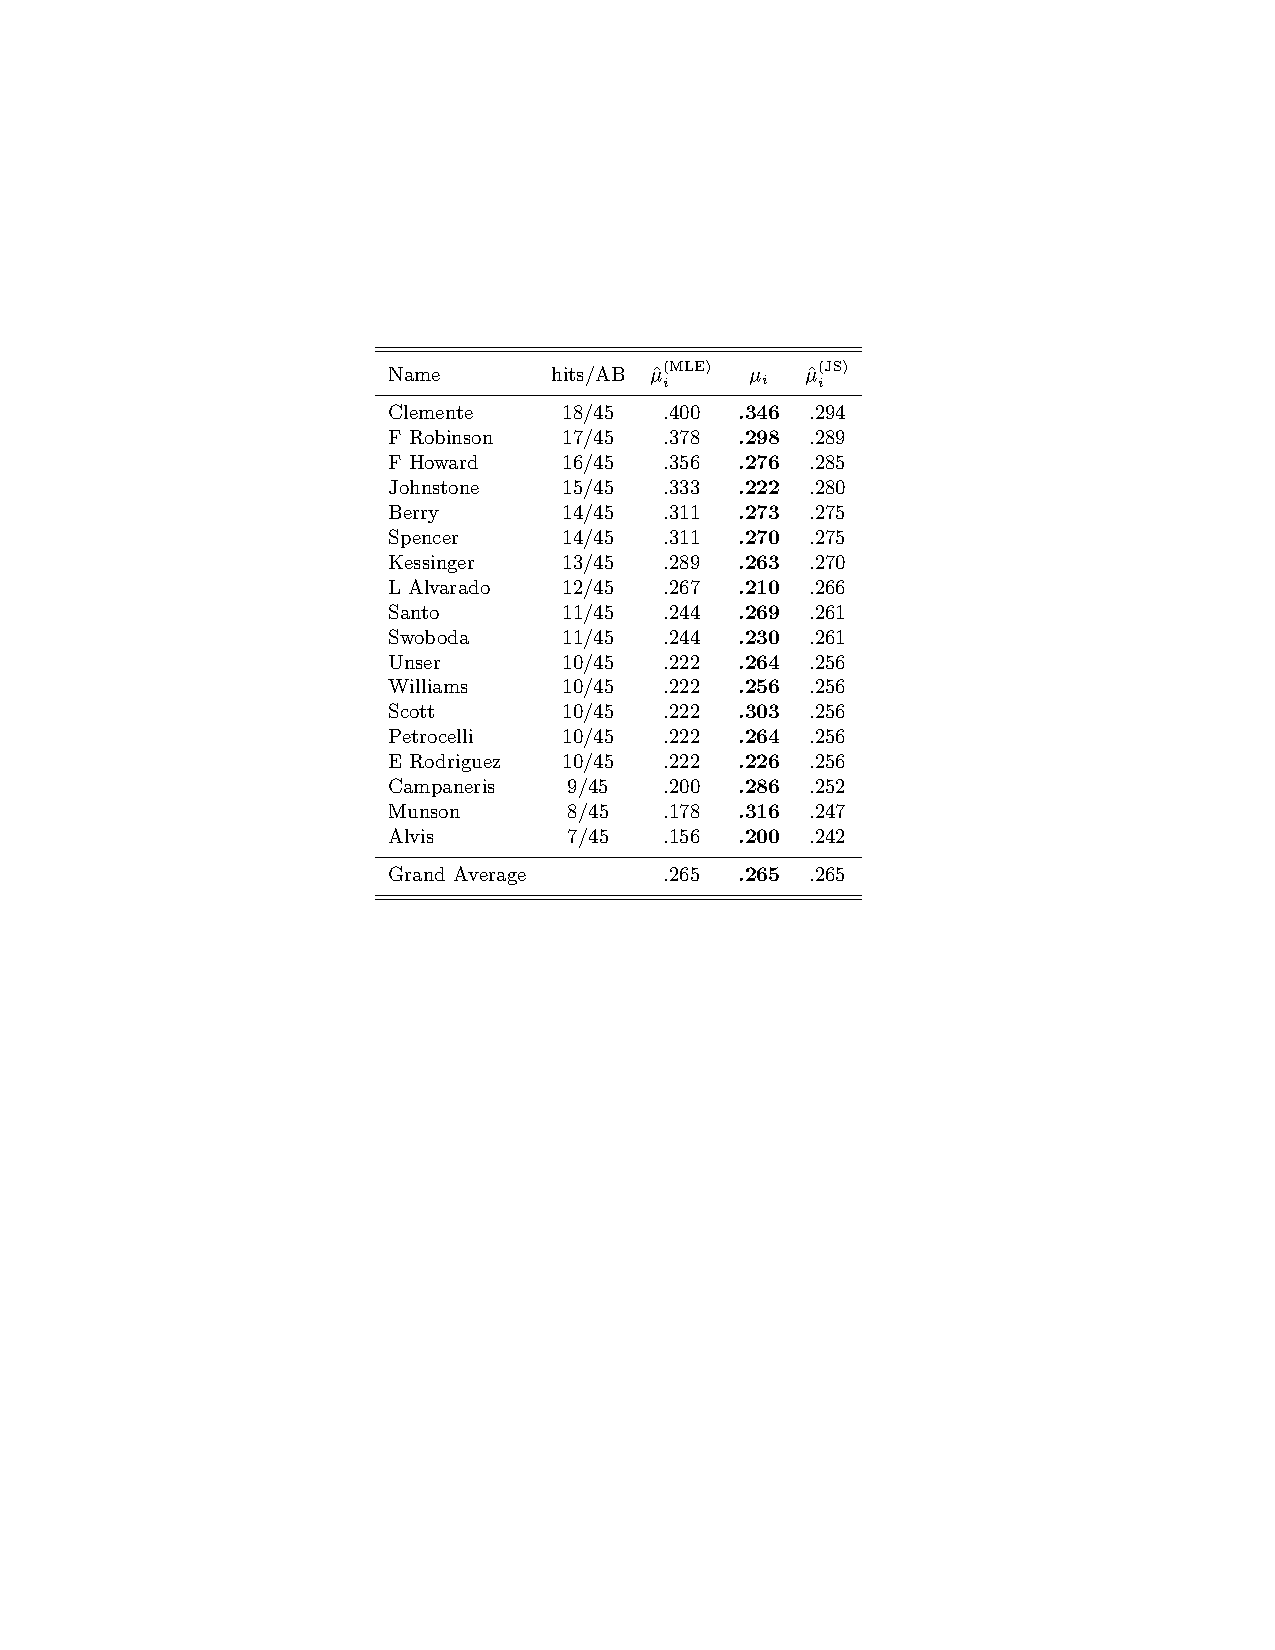
\includegraphics[height=0.8\textheight]{figures/JS_better}
	\end{minipage}%
	\begin{minipage}{.55\textwidth}
		\begin{itemize}
			\item
				Obviously, the MLE estimator is the early game average.
			\item
				JS estimator improves the estimation by a lot.
				The mean-square error ratio of JS estimation and MLE is
				about $0.28$, a signifiant reduction of total error.
			\item
				But what is the problem of JS estimator?
		\end{itemize}
	\end{minipage}
\end{frame}

\begin{frame}{}
	\centerline{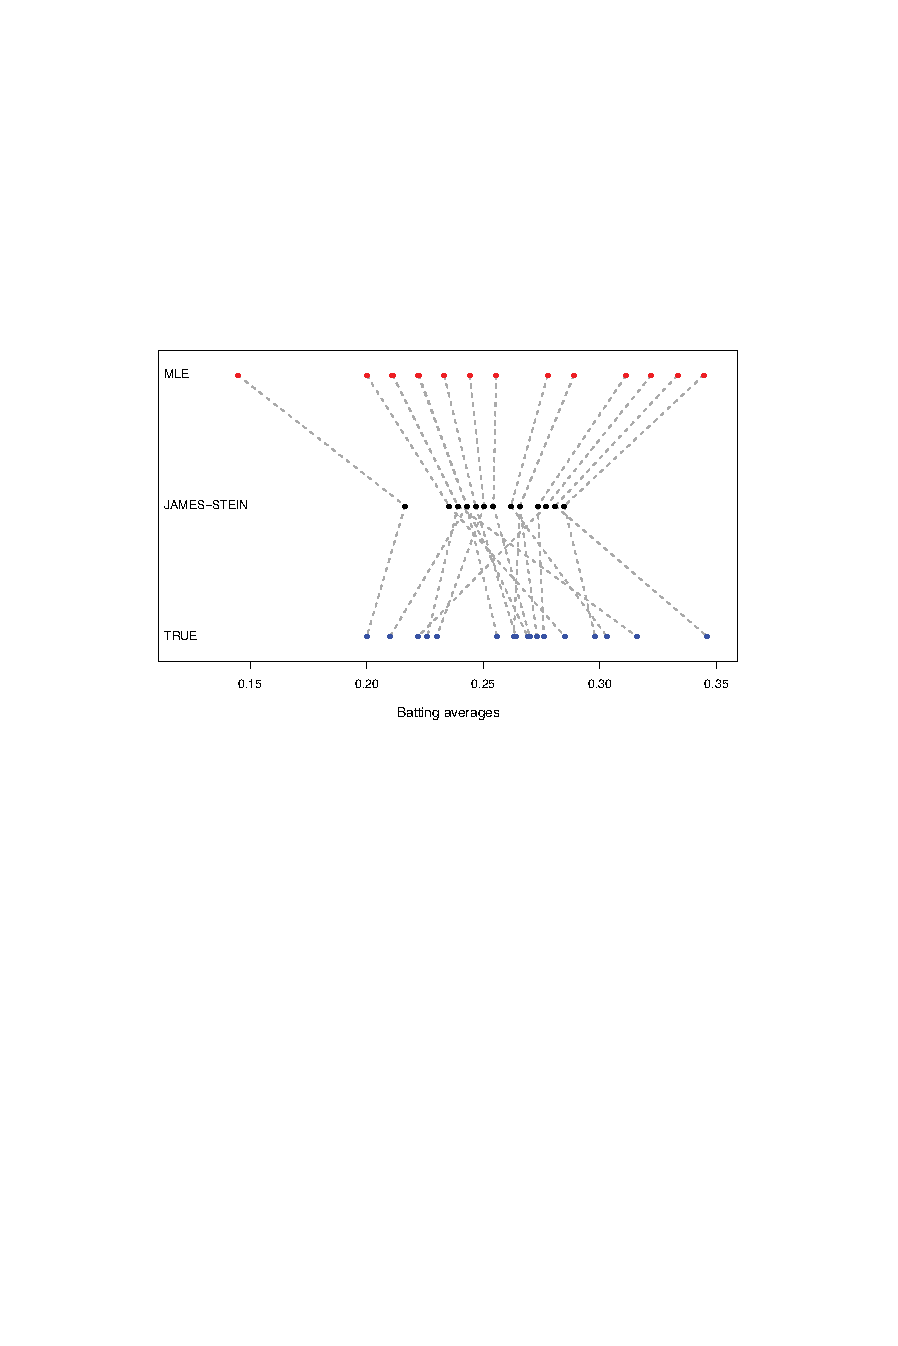
\includegraphics[height=0.8\textheight]{figures/visual}}
	JS estimator over shrink the estimates,
	and it is a poor estimator for extreme values.
\end{frame}

\begin{frame}{}
	\begin{minipage}{.5\textwidth}
		\noindent\hspace{-0.6cm}
		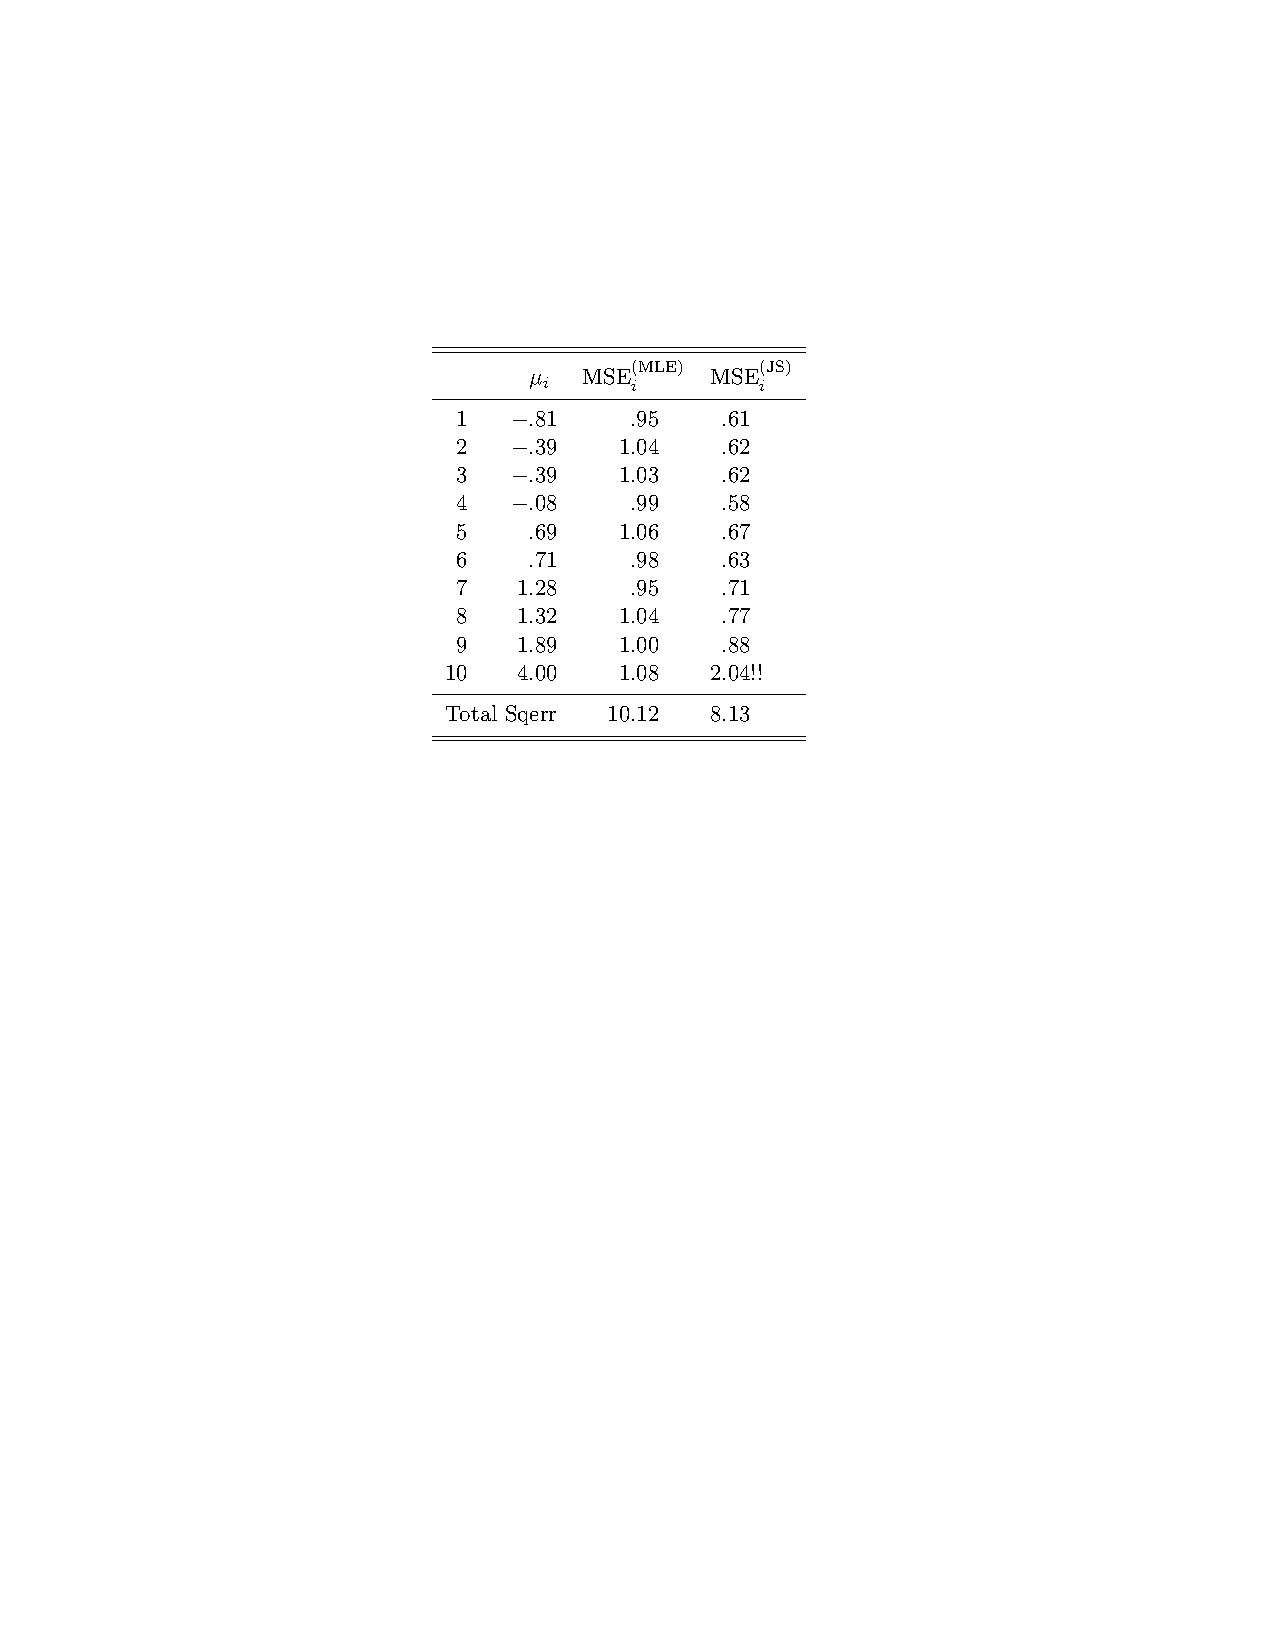
\includegraphics[height=0.8\textheight]{figures/JS_bad}
	\end{minipage}%
	\begin{minipage}{.55\textwidth}
		\begin{itemize}
			\item
				Left chart is created through simulations with
				$\bfz\given\bfmu\sim\normal[10]{\bfmu,I}$.
			\item
				Notice that although the total error improves under JS
				estimator, but individual estimation sufferers from the
				shrinkage.
			\item
				Traditional statistical methods are conservative in
				protecting individual effects from the tyranny of the majority,
				while JS estimator does not.
		\end{itemize}
	\end{minipage}
\end{frame}

\subsection{Remarks on JS estimator}

\begin{frame}{}
	\begin{itemize}
		\item
			However, sacrificing individual performance does imply a better
			performance over all.  In cases of large scale inferences, a better
			overall performance is favoured.
		\item
			If we insist on preserving some correctness of individual
			inferences, compromising methods are available.  One such
			compromising method is to choose MLE (adjusted with overall s.d.)
			whenever the JS estimator and MLE disagree too much.
			This method is call \emph{Limited translation estimates},
			developed by Efron \& Morris in the 1970s.
		\item
			JS estimator are also applied to adjust regression results and
			construct confidence intervals.  More methods, throughout the
			years, are introduced to ``generalized'' the result of JS
			estimator.
		\item
			In fact, Stein proved that MLE is inadmissible before proposing
			the JS estimator.
			He also proved that JS estimator itself is also inadmissible,
			but no explicit form has been found.
	\end{itemize}
\end{frame}

\section{Conclusion}

\begin{frame}{Conclusion}
	James and Stein not only introduced an estimator that dominates MLE in high
	dimension inference, the JS estimator also inspired other modern
	statistical methods through the following two ways:
	\begin{enumerate}
		\item \textbf{Learning from the experience of others}:
			This is a borrowing from Bayesian statistics into Frequentists'
			arsenal: the idea that estimation can be improved using
			``indirect evidence.''
			Later employed into \emph{large scale hypothesis testing} and
			\emph{false discovery rate control}.
		\item \textbf{Shrinkage}:
			The \emph{shrinkage principle} and \emph{bias-variance trade-off}
			are perhaps the two of the most influential ideas in modern day
			statistics and machine learning.  Lasso, Ridge, and other
			regulation methods in regression are now common place.
			\hfill$\blacksquare$
	\end{enumerate}
\end{frame}

\begin{frame}{References}
	\begin{enumerate}
		\item
			Efron, B. (2010).
			\textit{Empirical Bayes and the James—Stein Estimator.}
			Large-Scale Inference:
			Empirical Bayes Methods for Estimation, Testing, and Prediction
			(Institute of Mathematical Statistics Monographs, pp. 1-14).
			Cambridge: Cambridge University Press.
			doi: \url{https://doi.org/10.1017/CBO9780511761362.002}
		\item
			Efron, B., \& Morris, C. (1977).
			\textit{Stein's Paradox in Statistics.}
			Scientific American, 236(5), 119-127.
			Retrieved from \url{http://www.jstor.org/stable/24954030}
	\end{enumerate}
\end{frame}

\end{document}
